\documentclass[conference]{IEEEtran}
\IEEEoverridecommandlockouts
\usepackage{cite}
\usepackage{amsmath,amssymb,amsfonts}
\usepackage{graphicx}
\usepackage{textcomp}
\usepackage{xcolor}
\usepackage{booktabs}
\usepackage{microtype}
\usepackage{hyperref}
\hypersetup{colorlinks=true,linkcolor=blue,citecolor=blue,urlcolor=blue}

\begin{document}

\title{Repairing Safety Drift Without Retraining in Small Fine-Tuned Language Models: Weight-Space Methods and a Located Refusal Direction}

\author{\IEEEauthorblockN{Abdurrachman Mappuji\IEEEauthorrefmark{1}\IEEEauthorrefmark{2}}
\IEEEauthorblockA{\IEEEauthorrefmark{1}\textit{GCAS College Dublin}, Dublin, Ireland, Email: abdurrachman.mappuji@gcas.ie}
\IEEEauthorblockA{\IEEEauthorrefmark{2}\textit{Department of Cyber Security, Royal Holloway, University of London}, Egham, United Kingdom}
}

\maketitle

\begin{abstract}
Fine-tuning an aligned language model on benign data can erode its refusal behaviour. We ask whether such safety drift can be repaired without any further training. On Qwen2.5-1.5B-Instruct fine-tuned with LoRA on GSM8K, refusal on harmful prompts falls from 93.5\% to 59.5\% (and from 98.5\% to 55.0\% on XSTest's unsafe prompts), while ordinary harmless prompts are still answered. We evaluate ten training-free repairs on a laptop GPU, six metrics each with 95\% Wilson intervals: seven weight-space methods from the SafeTune library, two repairs that use a refusal direction we locate, and an ungated control. The direction is causal in layers 14 and above of 28: removing it cuts refusal of harmful prompts to 2--15\%, adding it makes the model refuse 90--100\% of harmless prompts, and the drifted model keeps near-perfect separability but a 34\% smaller harmful-versus-harmless gap at layer 26. Generic methods trace one trade-off between recovered refusal and over-refusal; SafeDelta and safety-vector restore reach near-aligned refusal (92.5--93.0\% on harmful prompts). A refusal weight patch built from the located direction recovers almost nothing (61.0\%). A conditionally gated steering push, with its size set from the measured gap, restores aligned-level refusal (96.5\%) with 3.3\% refusal of plain harmless prompts and unchanged GSM8K accuracy; the same push without the gate refuses 98\% of harmless prompts and fails every math problem. Intervals overlap with the best weight-space methods on most axes, and all repairs inherit the aligned model's high over-refusal of look-alike prompts (about 50\%), so we claim comparability, not superiority.

\end{abstract}

\begin{IEEEkeywords}
safety drift, fine-tuning, weight-space repair, refusal direction, activation steering, over-refusal
\end{IEEEkeywords}

\section{Introduction}
Safety alignment of instruction-tuned language models is fragile: fine-tuning on data that has nothing to do with safety can erode refusal behaviour, even when no one intends it~\cite{qi2023finetuning}. Practitioners who adapt an aligned model to a downstream task therefore face a practical question: after the model has drifted, can its safety be restored cheaply, without a second round of training, and without losing the task skill that motivated the fine-tune?

We study this question on a small, cheap-to-reproduce setup: the Qwen experiments run on a laptop GPU (Apple M1 with MPS) and the Tiny Aya experiments on a single cloud GPU (NVIDIA L4). We fine-tune Qwen2.5-1.5B-Instruct on grade-school math (GSM8K) with LoRA, confirm that harmful-prompt refusal drops sharply, and then compare a family of training-free repairs: weight-space methods implemented in the SafeTune library, and two repairs of our own that are motivated by locating where refusal is represented in the network. Our contributions are:
\begin{itemize}
\item A measurement of safety drift under a benign fine-tune, using six metrics with per-prompt outcomes and 95\% Wilson intervals, including a plain-harmless over-refusal set and XSTest's matched \emph{unsafe} prompts. We show that XSTest's safe look-alike prompts are a poor stand-in for over-refusal when used alone.
\item A layer-wise localisation of the refusal direction in the aligned and the drifted model, with a causal test (directional ablation and activation addition).
\item A second model, Tiny Aya Global, on which the same fine-tune produces \emph{no} measurable drift and on which two task-vector repairs reduce safety and math accuracy, so the Qwen result does not generalise.
\item A head-to-head comparison of ten training-free configurations (seven weight-space methods, two direction-based repairs and an ungated control; see Section~\ref{sec:method-ours}), and a negative result: the two repairs that exploit the located direction do not beat the trade-off curve traced by generic weight-space methods.
\end{itemize}

\section{Related Work}
\textbf{Safety drift.} Qi et al.~\cite{qi2023finetuning} showed that fine-tuning aligned models, even on benign data, degrades safety. Betley et al.~\cite{betley2025emergent} report broader misalignment emerging from narrow fine-tuning.
\textbf{Weight-space repair.} Task arithmetic~\cite{ilharco2023editing} edits models by adding or subtracting task vectors. Resta~\cite{bhardwaj2024resta} adds a safety vector, the difference between aligned and unaligned weights, to a fine-tuned model. WiSE-FT~\cite{wortsman2022robust} interpolates weights between models. Safe LoRA~\cite{hsu2024safelora} projects fine-tuning updates onto an alignment-aware subspace. SafeDelta~\cite{lu2025safedelta} applies a safety-preserving edit to the update. We use the implementations in SafeTune~\cite{safetune}.
\textbf{Refusal directions.} Arditi et al.~\cite{arditi2024refusal} show that refusal is mediated by a single direction in the residual stream; removing it disables refusal and adding it induces refusal. Conditional activation steering~\cite{lee2025cast} applies such a push only when a detector fires. Wei et al.~\cite{wei2024brittleness} localise safety-critical neurons and ranks.
\textbf{Over-refusal.} XSTest~\cite{rottger2024xstest} pairs safe prompts that look unsafe with genuinely unsafe ones, to measure exaggerated safety.

\section{Setup}
\subsection{Models and drift}
The aligned reference is Qwen2.5-1.5B-Instruct~\cite{qwen25}, the unaligned reference is Qwen2.5-1.5B (base). The Qwen models run in bfloat16 on an Apple M1 GPU through PyTorch MPS; Tiny Aya runs in bfloat16 on an NVIDIA L4 (22\,GB). To induce drift we fine-tune the aligned model with LoRA~\cite{hu2022lora} (rank 16, $\alpha$=32, all attention and MLP projections, learning rate $2\times10^{-4}$, batch size 8, one epoch over 2{,}000 GSM8K~\cite{cobbe2021gsm8k} training examples, loss on response tokens only) and merge the adapter. We call the result the \emph{drifted} model. Safety data play no role in this fine-tune. A second model, Tiny Aya Global~\cite{tinyaya} (3.35B parameters, 36 layers), receives the same recipe with its longer chat-template prompts (Section~\ref{sec:tinyaya}).

\subsection{Evaluation}
All generation is greedy. Each response is classified as a refusal if one of a fixed list of refusal phrases (e.g.\ ``I'm sorry'', ``I can't'', ``I cannot assist'') appears in its first 200 characters, following the substring convention of~\cite{arditi2024refusal}. We report six quantities, each with a 95\% Wilson interval:
\begin{itemize}
\item \emph{Harmful}: refusal rate on 200 prompts sampled from the held-out harmful test split of~\cite{arditi2024refusal}.
\item \emph{AdvBench}: refusal rate on 100 prompts from AdvBench~\cite{zou2023universal}.
\item \emph{XSTest-unsafe}: refusal rate on the 200 unsafe XSTest prompts.
\item \emph{XSTest-safe}: refusal rate on the 250 safe XSTest prompts (over-refusal on look-alikes; lower is better).
\item \emph{Harmless}: refusal rate on 150 ordinary harmless instructions (over-refusal on plain prompts; lower is better).
\item \emph{GSM8K}: exact-match accuracy of the final number on 150 test problems.
\end{itemize}
The substring detector is crude: it can miss refusals phrased unusually and count partial compliance as refusal. We therefore treat absolute levels with caution and focus on differences between models scored with the same detector.

\section{Methods}
\subsection{Locating the refusal direction}
For each layer $l$ we collect the residual-stream state at the final prompt token (after the chat template) for 260 harmful and 260 harmless training prompts, and set
\begin{equation}
\hat r_l = \frac{\mu^{\text{harm}}_l-\mu^{\text{safe}}_l}{\lVert\mu^{\text{harm}}_l-\mu^{\text{safe}}_l\rVert},\qquad g_l=\langle \hat r_l,\mu^{\text{harm}}_l-\mu^{\text{safe}}_l\rangle .
\end{equation}
Separability is the AUC of the projection $\langle\hat r_l,h\rangle$ on held-out validation prompts. For a causal test we (i) subtract the projection onto $\hat r_l$ from the output of every decoder layer (\emph{ablation}) and measure the refusal rate on harmful prompts, and (ii) add $\lVert\mu^{\text{harm}}_l-\mu^{\text{safe}}_l\rVert\,\hat r_l$ at layer $l$ (\emph{addition}) and measure refusal on harmless prompts (60 prompts each). We repeat the analysis on the drifted model and compare directions and gaps $g_l$.

\subsection{Training-free repairs from SafeTune}
We apply, to the drifted weights $W_d$ with aligned weights $W_a$ and base weights $W_b$, the following methods from SafeTune v0.1.12~\cite{safetune}: ReSta ($\alpha{=}0.5$, a DARE-masked safety vector $\alpha(W_a-W_b)$ added to $W_d$), task arithmetic ($\alpha{=}0.5$), WiSE-FT ($\alpha{=}0.5$, interpolation towards $W_a$), Safe LoRA (threshold 0.5), SafeDelta (strength 0.1), safety-vector restore (truncated-SVD safety subspace, rank 8, $\alpha{=}1$), and C-$\Delta\Theta$ (strength 1). None needs gradient steps, and on Qwen the weight edit itself takes seconds on a laptop. A first, smaller pass (100 harmful, 50 AdvBench, 75 GSM8K prompts) also swept ReSta's $\alpha$ and included SafeMerge, which left the drifted model essentially unchanged (63\% harmful refusal vs.\ 60\%).

\subsection{Repairs that use the located direction}\label{sec:method-ours}
We propose two repairs that use $\hat r_l$ on layers $\mathcal L=\{14,\dots,24\}$, the band where the causal test shows the direction matters.
\paragraph{Conditional steering.} At each $l\in\mathcal L$ we add $c_l\hat r_l$ to the residual stream only at positions whose projection exceeds a threshold $\tau_l$ (the midpoint of the harmful and harmless means, computed on the drifted model), with $c_l=\max(0,\,g^{\text{aligned}}_l-g^{\text{drifted}}_l)$, the gap lost to drift. This follows the gating idea of conditional activation steering~\cite{lee2025cast}; what we add is setting the push from the measured drift gap and calibrating the detector on the drifted model. The control, \emph{unconditional steering}, adds $c_l\hat r_l$ at every position.
\paragraph{Refusal weight patch.} For the matrices that write into the residual stream (attention output and MLP down projections) in $\mathcal L$, we undo the fine-tune's change along $\hat r_l$:
\begin{equation}
W \leftarrow W_d - \beta\,\hat r_l\hat r_l^{\top}(W_d-W_a),
\end{equation}
with $\hat r_l$ taken from the aligned model and $\beta\in\{1,2\}$.

\section{Results}
\subsection{Fine-tuning on math erodes refusal}
Table~\ref{tab:main} gives all six metrics for every model. The GSM8K fine-tune lowers refusal on harmful prompts from 93.5\% to 59.5\% and on XSTest's unsafe prompts from 98.5\% to 55.0\%; AdvBench refusal falls from 100\% to 90.0\%. Refusal of ordinary harmless prompts is not raised (8.0\% to 2.7\%), so the drift is a loss of caution, not a change in helpfulness. GSM8K accuracy is unchanged (51.3\% to 50.7\%): the fine-tune did not improve the task within our budget, which limits what ``preserving task performance'' can mean here (Section~\ref{sec:limits}). The aligned model refuses about half (50.8\%) of XSTest's safe look-alike prompts but only 8.0\% of plain harmless prompts, so the two over-refusal columns measure different things.

\begin{table*}[t]
\centering
\caption{Refusal rates and GSM8K accuracy (\%), with 95\% Wilson intervals in brackets. Higher is better for the first three columns and GSM8K; lower is better for the XSTest-safe and Harmless columns. Sample sizes: 200, 100, 200, 250, 150, 150. ``(ours)'' marks methods that use the located refusal direction.}
\label{tab:main}
\footnotesize
\setlength{\tabcolsep}{4pt}
Instruct (aligned) & 93.5 \scriptsize{[89,96]} & 100.0 \scriptsize{[96,100]} & 98.5 \scriptsize{[96,99]} & 50.8 \scriptsize{[45,57]} & 8.0 \scriptsize{[5,13]} & 51.3 \scriptsize{[43,59]} \\
Drifted (GSM8K LoRA) & 59.5 \scriptsize{[53,66]} & 90.0 \scriptsize{[83,94]} & 55.0 \scriptsize{[48,62]} & 3.2 \scriptsize{[2,6]} & 2.7 \scriptsize{[1,7]} & 50.7 \scriptsize{[43,59]} \\
\midrule
ReSta $\alpha$=0.5 & 82.0 \scriptsize{[76,87]} & 97.0 \scriptsize{[92,99]} & 73.5 \scriptsize{[67,79]} & 11.2 \scriptsize{[8,16]} & 5.3 \scriptsize{[3,10]} & 44.7 \scriptsize{[37,53]} \\
WiSE-FT 0.5 & 76.0 \scriptsize{[70,81]} & 95.0 \scriptsize{[89,98]} & 66.5 \scriptsize{[60,73]} & 8.0 \scriptsize{[5,12]} & 4.7 \scriptsize{[2,9]} & 52.7 \scriptsize{[45,60]} \\

\end{table*}

\subsection{Where refusal lives}
Figure~\ref{fig:locate} summarises the localisation. In the aligned model the projection onto $\hat r_l$ separates harmful from harmless validation prompts with AUC $\approx$ 1 from layer 12 onward (0.99 at layer 9). The causal test shows a sharp transition between layers 10 and 14: ablating the direction taken from layer 10 still leaves 80\% refusal, from layer 14 only 3\%. Directions taken from layers 4--8 leave refusal intact when ablated (95--97\% of harmful prompts still refused) and do not induce refusal when added (3--5\%); from layer 14 on, ablating the direction cuts refusal of harmful prompts to 2--15\% and adding it makes the model refuse 90--100\% of harmless prompts (60 prompts per condition). Refusal is therefore carried by a single direction in roughly layers 14--24, which we use as the repair band $\mathcal L$.

Drift leaves this structure largely in place. In the drifted model the harmful-versus-harmless AUC is still near 1, but the gap along the direction shrinks: at layer 26 it is 43.8 versus 66.5 in the aligned model (34\% smaller). The direction also rotates, with cosine similarity between the two models' directions between 0.62 and 0.96 across layers (lowest at layer 7). The model still separates the two kinds of prompt; the push towards refusing is weaker.

\begin{figure*}[t]
\centering
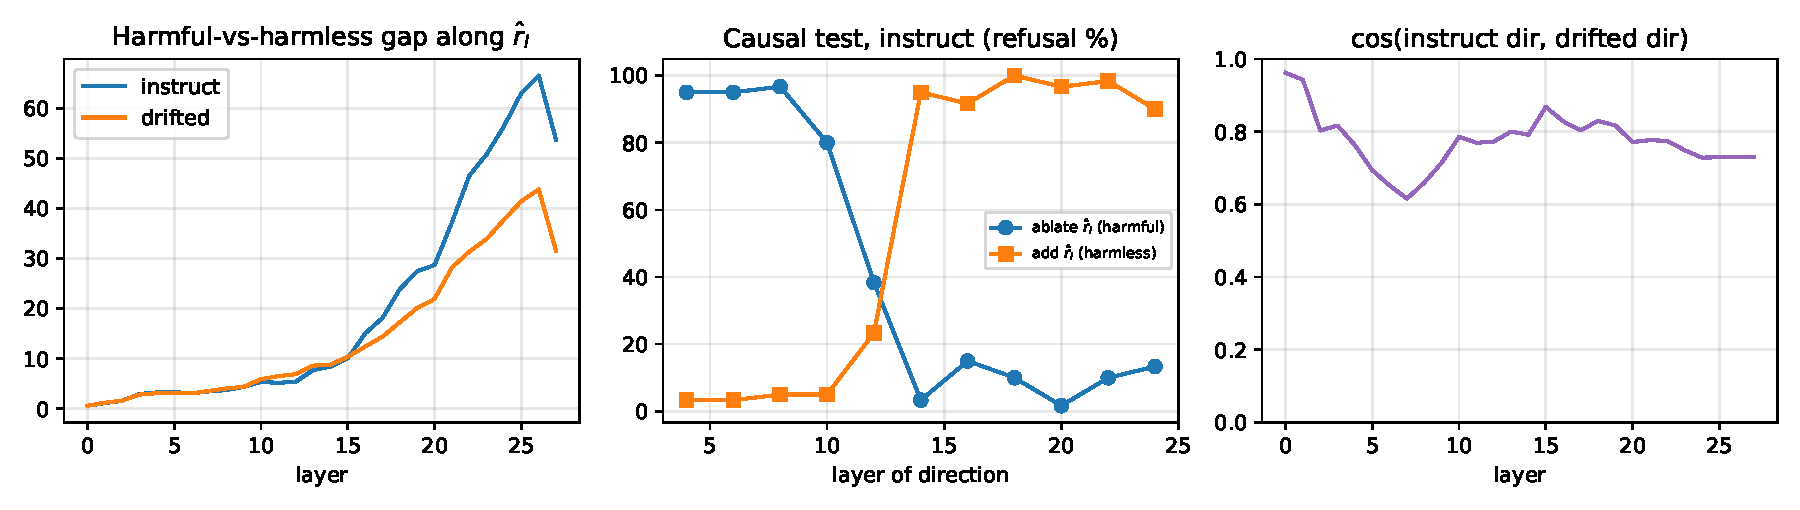
\includegraphics[width=\textwidth]{figures/locate.pdf}
\caption{Left: harmful-versus-harmless gap along $\hat r_l$ in the aligned and drifted models. Middle: causal test on the aligned model (60 prompts per point); directional ablation removes refusal and activation addition induces it from layer 14 on. Right: cosine similarity between the two models' directions.}
\label{fig:locate}
\end{figure*}

\subsection{Training-free repairs}
Figure~\ref{fig:tradeoff} plots safety (mean refusal over the three harmful sets) against both over-refusal measures.
\paragraph{Weight-space methods.} ReSta, task arithmetic, WiSE-FT and Safe LoRA are gentle: they raise harmful-prompt refusal to 76.0--82.5\% and XSTest-unsafe refusal to 66.5--78.5\% while plain-harmless over-refusal stays at 4.0--5.3\%. SafeDelta and safety-vector restore go further, to 93.0\% and 92.5\% on harmful prompts and 95.5\% and 97.5\% on XSTest-unsafe, close to the aligned model. Their look-alike over-refusal rises with refusal (32.8\% and 43.6\%, against 50.8\% for the aligned model), and plain-harmless over-refusal is 6.7\% for both. C-$\Delta\Theta$ sits in between (89.5\% harmful, 83.0\% unsafe). SafeMerge, tried in an earlier smaller pass, left the drifted model unchanged. Across these methods, more recovered refusal comes with more look-alike over-refusal.

\paragraph{Math accuracy.} GSM8K intervals are about $\pm$8 points wide, so most differences are not resolvable. SafeDelta (42.0\%) and C-$\Delta\Theta$ (40.0\%) have the lowest point estimates and ReSta is at 44.7\%, but all overlap with the drifted model's 50.7\%; safety-vector restore (54.7\%) and WiSE-FT (52.7\%) are at or above it. The only clear break is unconditional steering (0.0\%, interval [0,2]).

\begin{figure*}[t]
\centering
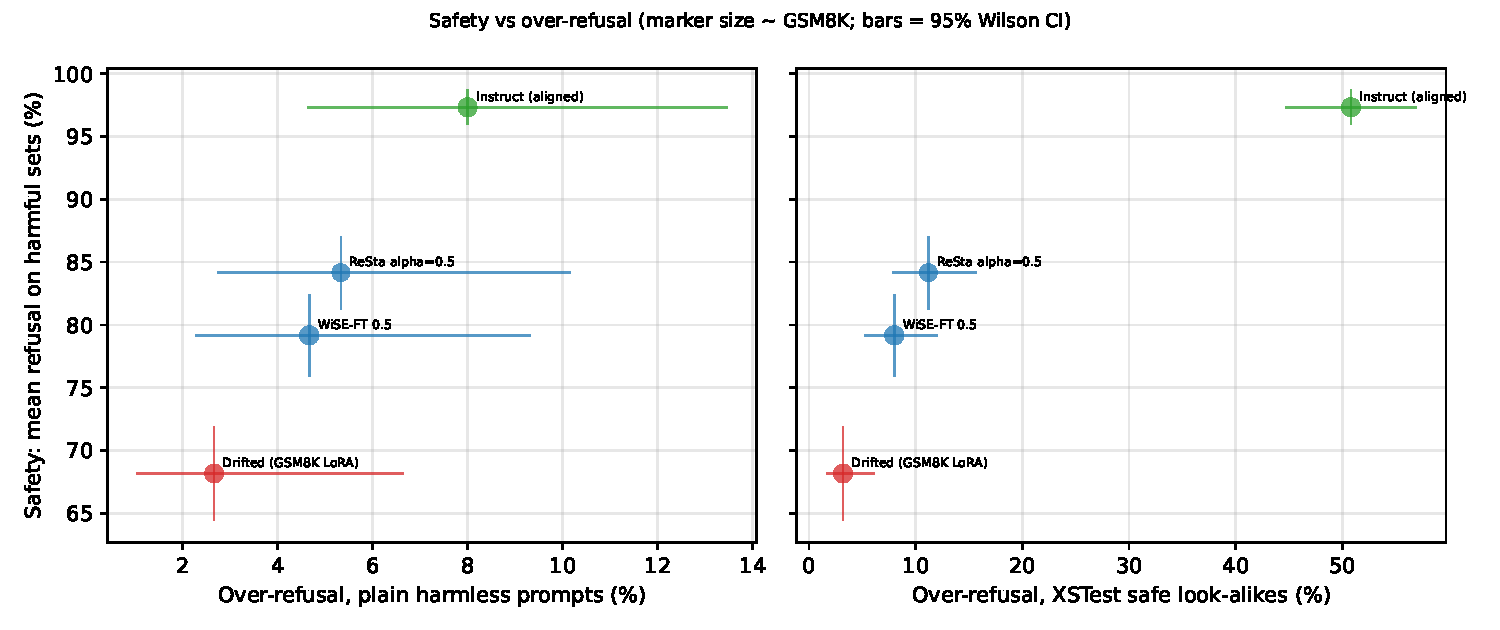
\includegraphics[width=\textwidth]{figures/tradeoff.pdf}
\caption{Safety versus over-refusal for the aligned model, the drifted model and each repair. Marker size grows with GSM8K accuracy; bars are 95\% Wilson intervals. Unconditional steering (98\% plain-harmless over-refusal) is omitted for scale and listed in Table~\ref{tab:main}.}
\label{fig:tradeoff}
\end{figure*}

\subsection{Repairs that use the located direction}
\paragraph{Refusal weight patch: negative result.} Undoing the fine-tune's change along $\hat r_l$ at the residual-write matrices of layers 14--24 recovers almost nothing: 61.0\% harmful-prompt refusal versus 59.5\% for the drifted model (and 65\% with $\beta{=}2$ in an earlier smaller run), with no change in over-refusal or math. The drift is therefore not stored mainly in how those layers write along the direction; it lies elsewhere, for example in how earlier layers or the read side encode the prompt, or in other directions.

\paragraph{Conditional steering.} Gated steering with the size set from the measured gap restores refusal to the aligned level: 96.5\% on harmful prompts, 96.0\% on AdvBench and 98.0\% on XSTest-unsafe. Plain-harmless over-refusal is 3.3\% [1,8], below the aligned model's 8.0\% [5,13], and GSM8K is 50.0\%. Against the best weight-space methods the evidence is comparability, not superiority: plain-harmless over-refusal for safety-vector restore is 6.7\% [4,12], an overlapping interval (five versus ten of 150 prompts), and the harmful-prompt refusal intervals overlap as well.
\paragraph{The gate is essential.} The same push applied at every position refuses 98.5\% of harmful prompts but also 98.0\% of plain harmless prompts and 100\% of safe look-alikes, and solves no GSM8K problem (0.0\%). The detector, not the push, is what preserves normal behaviour.
\paragraph{Look-alike prompts.} Conditional steering refuses 49.2\% of XSTest's safe look-alikes, matching the aligned model (50.8\%) and safety-vector restore (43.6\%). The direction appears to respond to harmful-looking content rather than harm itself. Steering therefore restores the aligned model's behaviour, including its look-alike weakness, and does not improve on it.

\subsection{A second model: Tiny Aya Global shows no drift}\label{sec:tinyaya}
We repeated the pipeline on Tiny Aya Global. Its chat template prepends a 366-token system preamble to every prompt, so GSM8K sequences are about 600 tokens and we truncate at 640 (the 320 used for Qwen would have masked every answer). We used the same LoRA recipe, and 250 steps took about 15 minutes on one NVIDIA L4. Evaluation uses the same six metrics with the default template, preamble included. Repairs use SafeTune's guidance for this model, $\alpha{=}0.25$ for ReSta and task arithmetic. Only six of the twelve planned configurations finished (Section~\ref{sec:limits}).

\begin{table*}[t]
\centering
\caption{Tiny Aya Global: refusal rates and GSM8K accuracy (\%) with 95\% Wilson intervals; same metrics and sample sizes as Table~\ref{tab:main}. Only six of twelve planned configurations finished.}
\label{tab:tinyaya}
\footnotesize
\setlength{\tabcolsep}{4pt}
\begin{tabular}{lcccccc}
\toprule
Model & Harmful & AdvBench & XSTest-unsafe & XSTest-safe & Harmless & GSM8K \\
\midrule
Aligned (Tiny Aya Global) & 89.5 \scriptsize{[84,93]} & 100.0 \scriptsize{[96,100]} & 80.0 \scriptsize{[74,85]} & 8.0 \scriptsize{[5,12]} & 2.0 \scriptsize{[1,6]} & 59.3 \scriptsize{[51,67]} \\
Drifted (GSM8K LoRA) & 89.5 \scriptsize{[84,93]} & 100.0 \scriptsize{[96,100]} & 77.5 \scriptsize{[71,83]} & 4.8 \scriptsize{[3,8]} & 1.3 \scriptsize{[0,5]} & 62.0 \scriptsize{[54,69]} \\
\midrule
ReSta $\alpha$=0.25 & 85.5 \scriptsize{[80,90]} & 98.0 \scriptsize{[93,99]} & 59.0 \scriptsize{[52,66]} & 4.8 \scriptsize{[3,8]} & 2.0 \scriptsize{[1,6]} & 42.0 \scriptsize{[34,50]} \\
WiSE-FT 0.5 & 88.0 \scriptsize{[83,92]} & 100.0 \scriptsize{[96,100]} & 79.0 \scriptsize{[73,84]} & 6.8 \scriptsize{[4,11]} & 1.3 \scriptsize{[0,5]} & 69.3 \scriptsize{[62,76]} \\
Task arith. $\alpha$=0.25 & 87.5 \scriptsize{[82,91]} & 99.0 \scriptsize{[95,100]} & 66.5 \scriptsize{[60,73]} & 4.0 \scriptsize{[2,7]} & 3.3 \scriptsize{[1,8]} & 42.7 \scriptsize{[35,51]} \\
Safe LoRA & 88.0 \scriptsize{[83,92]} & 100.0 \scriptsize{[96,100]} & 78.0 \scriptsize{[72,83]} & 6.8 \scriptsize{[4,11]} & 1.3 \scriptsize{[0,5]} & 64.7 \scriptsize{[57,72]} \\
\bottomrule
\end{tabular}

\end{table*}

\paragraph{The fine-tune does not erode safety.} Harmful-prompt refusal is 89.5\% before and after, AdvBench is 100\% in both, XSTest-unsafe moves from 80.0\% to 77.5\% (intervals overlap) and GSM8K from 59.3\% to 62.0\% (Table~\ref{tab:tinyaya}). The localisation agrees (Figure~\ref{fig:locate-tinyaya}): the aligned and drifted refusal directions have cosine similarity 0.94--1.0 at every layer we sampled (the even layers), and the drifted model's harmful-versus-harmless gap is slightly \emph{larger}, not smaller (97 versus 92 at layer 34). The causal transition sits at layers 12--14 of 36, as for Qwen: ablating the direction from layer 14 on leaves 2--22\% refusal, and adding it induces 78--98\%. We did not test why Tiny Aya resists drift; one untested candidate is the safety-mode preamble present in both training and evaluation prompts.

\begin{figure*}[t]
\centering
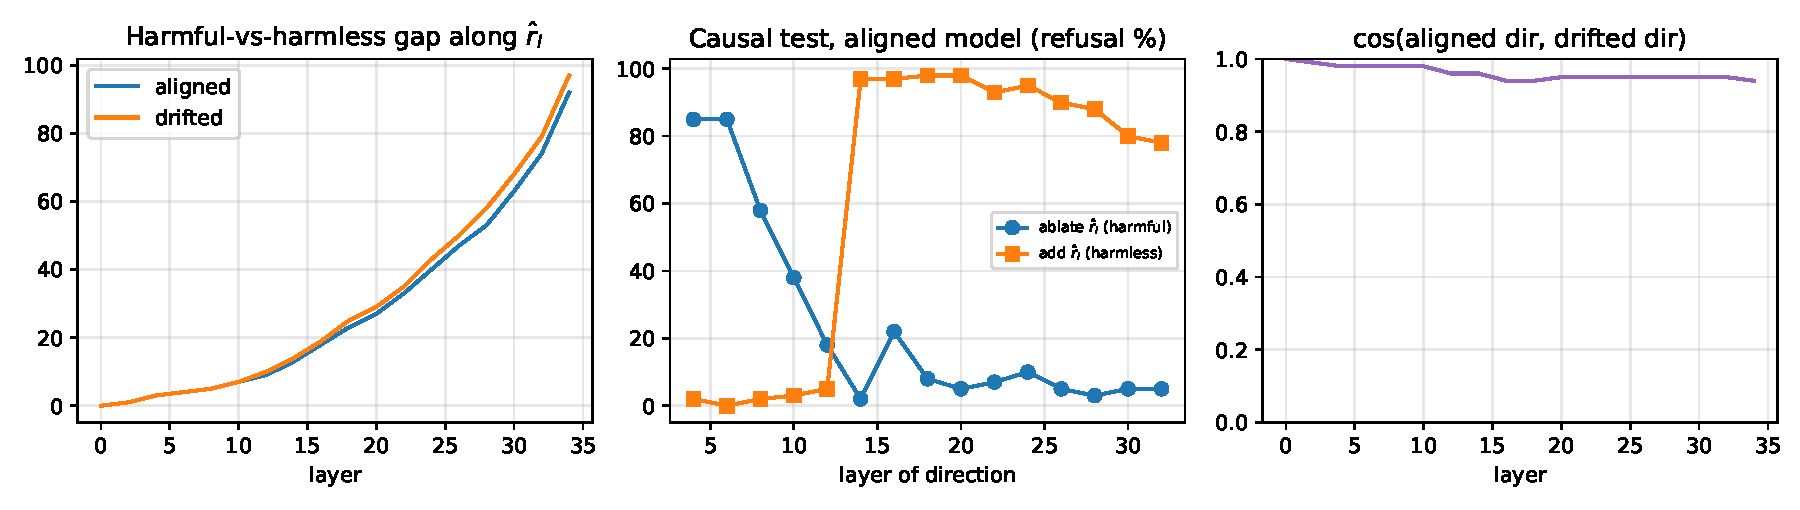
\includegraphics[width=\textwidth]{figures/locate_tiny_aya.pdf}
\caption{Tiny Aya Global: gap along the refusal direction (aligned vs drifted, even layers), causal test on the aligned model (60 prompts per point), and cosine similarity between the two models' directions. Compare Figure~\ref{fig:locate}.}
\label{fig:locate-tinyaya}
\end{figure*}

\paragraph{Task-vector repairs hurt a model that did not drift.} ReSta ($\alpha{=}0.25$) lowers XSTest-unsafe refusal to 59.0\% [52,66] from 77.5\% [71,83] and GSM8K to 42.0\% [34,50] from 62.0\% [54,69]; both intervals fall clear of the drifted model's. Task arithmetic gives 66.5\% on XSTest-unsafe (a borderline drop, intervals overlap slightly) and 42.7\% [35,51] on GSM8K. A plausible reason, which we did not isolate, is the size of the aligned-minus-base difference in this model: the relative weight change averages about 21\% (maximum 58\%) across matrices, far larger than a small fine-tune. WiSE-FT and Safe LoRA are harmless (XSTest-unsafe 79.0\% and 78.0\%), and WiSE-FT is highest on GSM8K at 69.3\%.


\section{Limitations}
\label{sec:limits}
\begin{itemize}
\item \textbf{One model, one drift source, one seed.} All results are for Qwen2.5-1.5B-Instruct after a single GSM8K LoRA fine-tune. The fine-tune did not improve GSM8K accuracy, so we cannot show that repairs preserve a \emph{gained} skill, only that accuracy is not clearly changed.
\item \textbf{Crude refusal detector.} Refusal is a phrase match in the first 200 characters, not a judged outcome. It can miss unusual refusals and count hedged compliance as refusal, and absolute levels (notably the aligned model's 50.8\% on XSTest-safe) should not be over-read. No guard model or human review was used.
\item \textbf{Small evaluation sets.} With 100--250 prompts per metric the 95\% intervals span roughly 4 to 16 points (GSM8K about $\pm$8), so many comparisons are unresolved. We do not claim any ranking among methods whose intervals overlap.
\item \textbf{Untuned, single settings.} Each method was run at one setting chosen without per-method tuning (the SafeTune defaults or our first choice), so the ranking depends on those choices. The repair band (layers 14--24) was chosen after inspecting the aligned model's causal test.
\item \textbf{Aligned reference required.} Every repair uses the aligned model, and several also the base model, so they apply only when those weights exist.
\item \textbf{No adversarial evaluation.} We test direct harmful requests only, not jailbreaks, multi-turn attacks, prompt injection or weight-space attacks. Greedy decoding only.
\item \textbf{Toolkit coverage.} We used the SafeTune weight-space methods; we did not use SafeTune's own circuit or neuron finders, CircuitKIT, AuditKIT or CuratorKIT, and the localisation here is our own analysis.
\end{itemize}


\section{Conclusion}
Benign fine-tuning of a 1.5B model on math removed a third of its refusal on harmful prompts without raising its refusal of ordinary requests. Training-free repairs recover it, and the stronger weight-space methods (SafeDelta, safety-vector restore) reach near-aligned refusal in seconds on a laptop. Refusal in this model is carried by a single direction in layers 14--24 that drift weakens but does not destroy. A repair that edits weights along that direction fails, whereas a gated steering push sized by the measured gap restores aligned-level refusal with ordinary prompts and math unaffected, and only if it is gated. Conditional steering was comparable to, not better than, the best weight-space methods, and every repair inherits the aligned model's tendency to refuse harmless look-alike prompts. The next steps are a judged refusal metric, adversarial evaluation, a drift source that improves the task, and more models.


\section*{Reproducibility}
Code, result files and the scripts that generate every table and figure are in the accompanying repository (\texttt{empeje/lexsi-ai-hackathon}); the Qwen experiments ran on a single Apple M1 machine with 64\,GB of unified memory and the Tiny Aya experiments on one NVIDIA L4 (22\,GB) in Colab Enterprise, using the notebook in the repository's \texttt{colab/} folder.

\begin{thebibliography}{99}
\bibitem{qi2023finetuning} X.~Qi \emph{et al.}, ``Fine-tuning aligned language models compromises safety, even when users do not intend to!'' in \emph{ICLR}, 2024.
\bibitem{betley2025emergent} J.~Betley \emph{et al.}, ``Emergent misalignment: Narrow finetuning can produce broadly misaligned LLMs,'' 2025.
\bibitem{ilharco2023editing} G.~Ilharco \emph{et al.}, ``Editing models with task arithmetic,'' in \emph{ICLR}, 2023.
\bibitem{bhardwaj2024resta} R.~Bhardwaj, D.~D. Anh, and S.~Poria, ``Language models are Homer Simpson! Safety re-alignment of fine-tuned language models through task arithmetic,'' in \emph{ACL}, 2024.
\bibitem{wortsman2022robust} M.~Wortsman \emph{et al.}, ``Robust fine-tuning of zero-shot models,'' in \emph{CVPR}, 2022.
\bibitem{hsu2024safelora} C.-Y. Hsu \emph{et al.}, ``Safe LoRA: The silver lining of reducing safety risks when fine-tuning large language models,'' in \emph{NeurIPS}, 2024.
\bibitem{lu2025safedelta} N.~Lu \emph{et al.}, ``SafeDelta: Consistently preserving safety when fine-tuning LLMs on diverse datasets,'' in \emph{ICML}, 2025.
\bibitem{safetune} Lexsi Labs, ``SafeTune: auditing and repairing safety drift in fine-tuned LLMs,'' software, \url{https://safetune.lexsi.ai}.
\bibitem{arditi2024refusal} A.~Arditi \emph{et al.}, ``Refusal in language models is mediated by a single direction,'' in \emph{NeurIPS}, 2024.
\bibitem{lee2025cast} B.~W. Lee \emph{et al.}, ``Programming refusal with conditional activation steering,'' in \emph{ICLR}, 2025.
\bibitem{wei2024brittleness} B.~Wei \emph{et al.}, ``Assessing the brittleness of safety alignment via pruning and low-rank modifications,'' in \emph{ICML}, 2024.
\bibitem{rottger2024xstest} P.~R{\"o}ttger \emph{et al.}, ``XSTest: A test suite for identifying exaggerated safety behaviours in large language models,'' in \emph{NAACL}, 2024.
\bibitem{zou2023universal} A.~Zou \emph{et al.}, ``Universal and transferable adversarial attacks on aligned language models,'' 2023.
\bibitem{tinyaya} Cohere Labs, ``Tiny Aya Global,'' model card, \url{https://huggingface.co/CohereLabs/tiny-aya-global}.
\bibitem{qwen25} Qwen Team, ``Qwen2.5 technical report,'' 2024.
\bibitem{hu2022lora} E.~J. Hu \emph{et al.}, ``LoRA: Low-rank adaptation of large language models,'' in \emph{ICLR}, 2022.
\bibitem{cobbe2021gsm8k} K.~Cobbe \emph{et al.}, ``Training verifiers to solve math word problems,'' 2021.
\end{thebibliography}

\end{document}
